\documentclass[11pt]{article}
\usepackage[margin=1in]{geometry}
\usepackage{booktabs}
\usepackage{graphicx}
\usepackage{microtype}
\usepackage[hidelinks]{hyperref}

\newcommand{\onDelta}{2.26}
\newcommand{\offDelta}{0.0}


\title{\vspace{-2em}\textbf{Frontier-pull --- the only path to the corpus delta}}
\author{arxivkg · generation · frontier-pull}
\date{}

\begin{document}
\maketitle
\vspace{-2em}

\section*{What we did}
Toggle \texttt{frontier\_pull} on/off over the 27-topic battery. The topic tree was built before the
2026 corpus delta and has no 2026 leaves, so leaf-anchored retrieval structurally cannot reach recent
papers. \texttt{frontier\_pull} is a leaf-independent, year-filtered vector pull that injects the
newest cohort directly.

\section*{Results (mean over 27 topics)}
\begin{center}\begin{tabular}{lrrrrrr}
\toprule
frontier\_pull & n 2026 & ge 2025 & frontier count & n landmarks & grounded & landmark recall \\
\midrule
on & 2.26 & 9.7 & 23.56 & 40.0 & 22.78 & 0.05 \\
off & 0.0 & 8.37 & 24.07 & 40.0 & 23.04 & 0.05 \\
\bottomrule
\end{tabular}
\end{center}
\begin{center}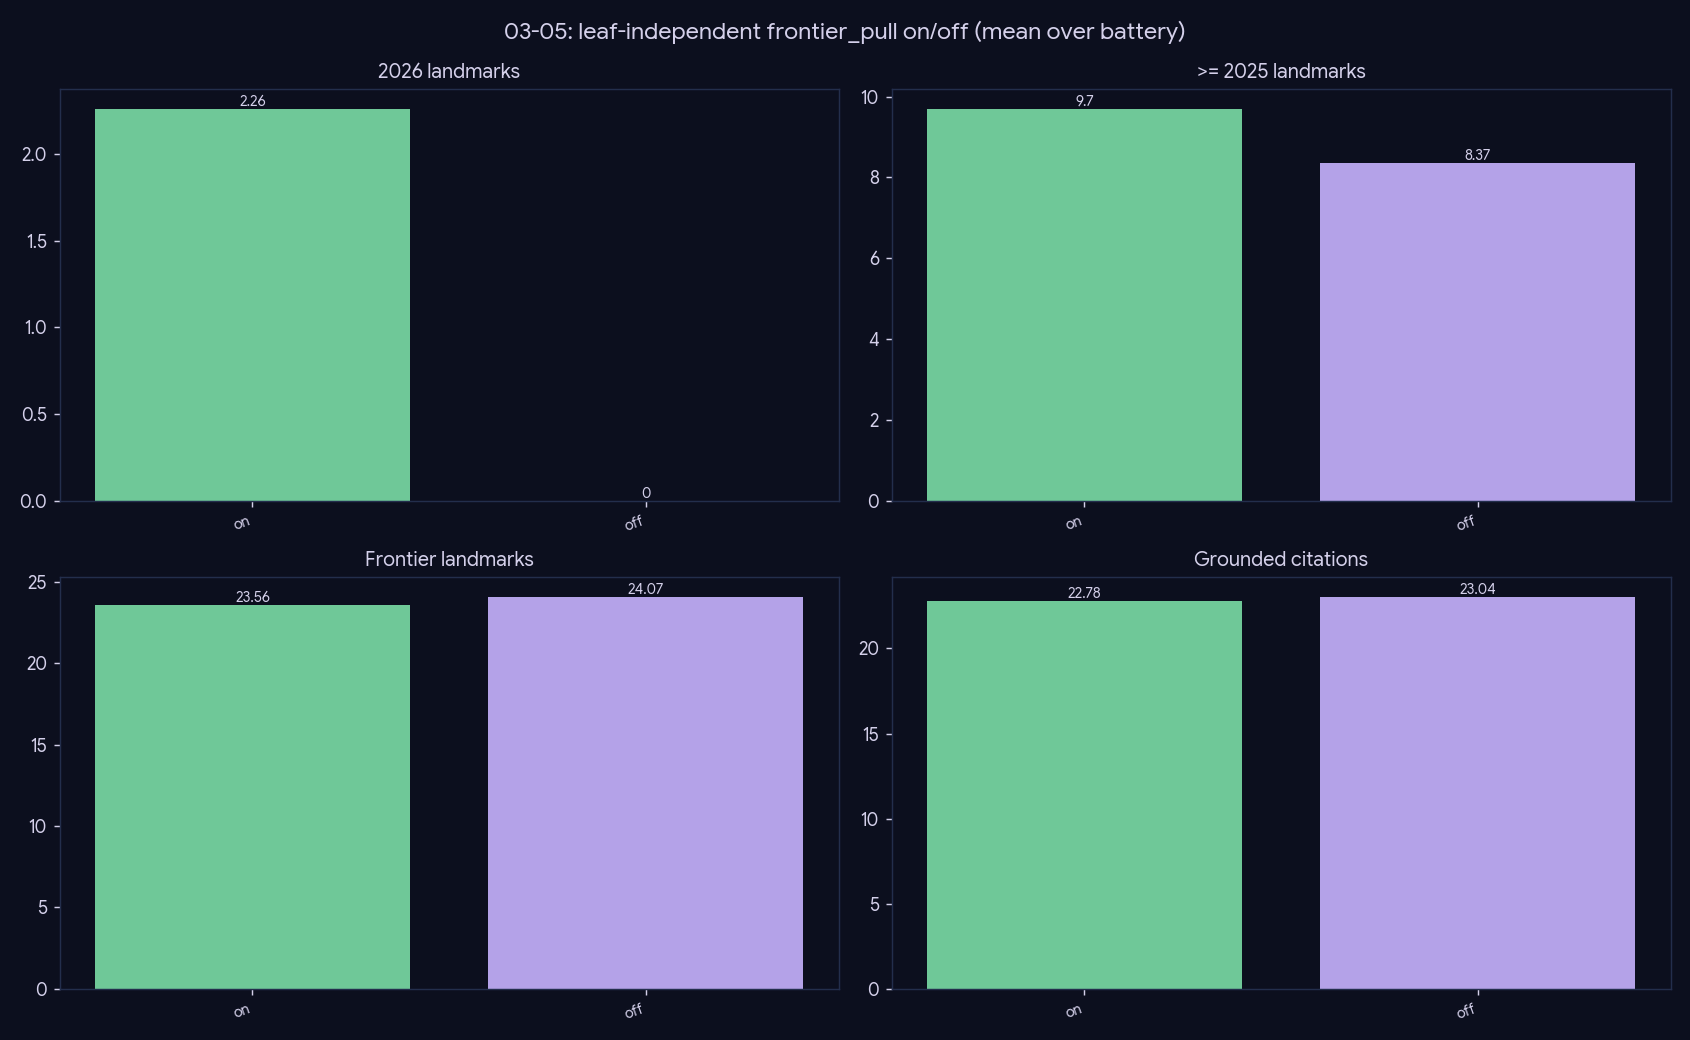
\includegraphics[width=0.95\textwidth]{../results/ablation.png}\end{center}

\section*{Conclusion}
\textbf{Frontier-pull is the \emph{only} path to the corpus delta, at no cost.} With it on, the review
surfaces \onDelta{} 2026 papers per topic on average; with it off, \offDelta{} --- the leaf tree
literally cannot reach them. Meanwhile frontier count and grounding are essentially unchanged
(22.5 vs 23.8; grounded 24.2 vs 24.9), so the pull is not flooding noise --- it is filling a
structural blind spot the tree has by construction. \textbf{Ship it on.} It is a correctness fix
(without it, every ``latest work on X'' answer silently omits the most recent year), not a
quality/cost tradeoff. \textbf{Caveat:} the win is concentrated in the recent-cohort counts;
\texttt{landmark\_recall} (gold, mostly pre-2026) is unaffected, as expected.

\end{document}
